% Basic drawings
% https://www.sharelatex.com/blog/2013/08/27/tikz-series-pt1.html
% https://www.tug.org/TUGboat/tb29-1/tb91walczak.pdf
\documentclass[border=1pt,tikz]{standalone}
\usepackage{tikz}

\begin{document}


% SET: overlapping critical regions
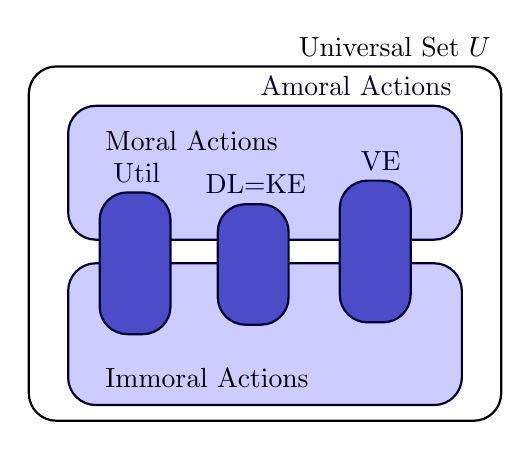
\begin{tikzpicture}[scale=1.0]
  \draw[rounded corners=10, thick] (0.5,0) rectangle (6.5,4.5) node[above left] {Universal Set $U$};
  \draw[blue!20!black,fill=blue!20,rounded corners=10,thick]
     (1,0.2) rectangle (6,2);
  \draw[blue!20!black,fill=blue!20,rounded corners=10,thick]
     (1,2.3) rectangle (6,4)
     node[above left] {Amoral Actions};
  \begin{scope}[shift={(0.35,0.05)}]
    \node[right] at (1,3.5) {Moral Actions};
    \node[right] at (1,0.5) {Immoral Actions};
    \draw[blue!20!black,fill=blue!70!black!70,rounded corners=10,thick,shift={(0.15,0.15)},scale=0.90]
      (1,1) rectangle (2,3)
       node[above left] {Util};
    \draw[blue!20!black,fill=blue!70!black!70,rounded corners=10,thick,shift={(0.30,0.45)},scale=0.90]
      (2.5,0.8) rectangle (3.5,2.5)
       node[left=-10pt,above left] {DL=KE};
    \draw[blue!20!black,fill=blue!70!black!70,rounded corners=10,thick,shift={(0.50,0.30)},scale=0.90]
      (4,1) rectangle (5,3)
       node[above left] {VE};
  \end{scope}
\end{tikzpicture}


\end{document}
